\section{Related Work}

The field of compute governance contains many proposals for regulations that implicitly rely on the ability to reliably identify when developers are using compute for AI training, and many proposals for hardware-enabled mechanisms that assist our classifier in securely providing that information. \citet{shavit2023} proposes compute monitoring for verifying rules on large-scale training. \citet{sastry2024} provide a comprehensive framework for compute as a governance lever. \citet{heimkoessler2024} analyse FLOP thresholds as a regulatory instrument; for example, the 10$^2$6-FLOP line in U.S. EO 14110 is a direct operationalisation of this. \citet{scher2025} propose an international agreement wherein training above certain compute thresholds is monitored and restricted or prohibited, while inference is allowed; this would require the ability to distinguish between inference and training on monitored hardware. \citet{baker2025} identify six verification layers for international AI agreements; our work provides empirical evidence for one layer (built-in monitoring). \citet{ogara2025} and the RAND workshop report \citep{kulp2025} evaluate HEM options including workload attestation. \citet{petriesolo2025} proposes firmware-based offline licensing for export controls. \citet{seferis2025} argue that compute-structuring evasion (splitting training across providers) is detectable conditional on per-host workload classification; we supply and stress-test exactly that per-host classifier. Differential Architecture \citep{anonymous2026} proposes hardware mechanisms to limit performance of targeted applications, a type of enforcement complementary to our detection approach. One possibility is to robustly classify all workloads on hardware within the governance jurisdiction, and then apply the differential architecture performance restrictions to automatically enforce the established rules.

There is also existing research relevant to workload classification, which we extend. \citet{monfared2026} study timing and memory observables for detecting training when host and device are untrusted, constructing their own derived signals from primitives that survive a strong tampering adversary. They establish signals that remain informative when NVML cannot be relied upon. Our case is complementary, establishing highly successful classification from signals that will be reliable if they can be protected from tampering by HEMs. Their work establishes a lower floor on the signal set; ours establishes an upper bound on what an adversary can hide inside that signal set. \citet{chen2025b} develop a hardware-centric, workload-agnostic approach to hardware monitoring, analyzing over 30 ML models on various hardware platforms to perform anomaly detection using an unsupervised learning pipeline. Our scope includes supervised examples, using more than 1400 labeled records of workloads totaling over 100 hours of hardware signal telemetry to teach the classifier to recognize ML training from those signals. \citet{gangwal2019} investigate a conceptually very similar problem, using hardware performance counters for workload classification using RF and SVM models, but with the objective of discovering covert cryptomining, not ML training. The study notes an adversarial limitation: they predicted that evasion may be possible by restricting mining operations to obfuscate the workload signature, but at a profitability cost, analogous to the throughput penalty that evaders would suffer while attempting to evade classifiers such as ours. We extend the workload classification objective to the adversarial setting, where operators attempt to deceive the classifier.

Other past work covers several adjacent but distinct tasks. WAVE \citep{xu2026} identify inference workloads with 87-93\% accuracy using 24 Nsight Compute per-kernel counters (1,200-5,300\% overhead). We accomplish a similar-granularity classification using only always-available NVML physical counters at zero runtime overhead; the tasks are not identical (WAVE separates inference families; we separate training from inference and others), so results are not directly comparable. \citet{esposito2025} combine NVML telemetry and performance counters to estimate GPU stress and reliability across workloads. Their results confirm that telemetry reveals meaningful workload differences, but the target is reliability estimation rather than governance-oriented training detection. ShadowScope \citep{almusaddar2025} uses composable performance-counter signals to detect anomalous behaviors and prevent attacks which could compromise the integrity of GPU computation. We collect and analyze similar data, but using NVML readings rather than CUDA profiling events.

Using physical side channels rather than software telemetry, \citet{maia2022} show magnetic flux from GPU power cables reveals neural network topology. \citet{arefin2025} demonstrate USB/HDMI port power measurement can infer GPU activities. \citet{latif2025} empirically measure power signatures of training on 8-GPU H100 nodes. These establish that physical signals carry workload-identifying information; we extend this to software-accessible telemetry for governance. POLCA \citep{patel2023} characterize LLM power consumption profiles across a Microsoft Azure fleet for energy planning and find systematic differences in power patterns between training and inference, providing independent evidence for the signal detected by our classifier, at the scale of large cloud datacenters.

\section{Classifier Design}
\label{sec:clfdesign}

\subsection{Deployed Classifier}

The operational form we deploy is a two-stage pipeline that factors the decision along a natural tree:

\begin{itemize}\itemsep2pt
  \item \textbf{Is the workload ML?} A binary RandomForest head using all features extracted from telemetry readings classifies the workload into \texttt{ml\_training} $\cup$ \texttt{ml\_inference} vs other. The ML-vs-non-ML boundary leans heavily on level signals (peak memory footprint, sustained tensor-core utilization, power draw), so the full feature set is retained.
  \item \textbf{If the workload is ML, is it training?} A binary RandomForest head trained only on records where the true category is training or inference classifies incoming readings into either category. This head receives a subset of features with level features dropped (absolute memory/power/clock means, percentiles, min, max, range). The train-vs-infer decision rests on shape, periodicity, FFT, and autocorrelation terms only. This prevents the classifier from overfitting to specific models previously tested and specific power, memory, or compute throughput levels associated with particular GPUs. This also makes the classifier more robust to certain adversarial strategies: for example, the evader cannot modulate their usage levels to match that of another chip that is specifically designed for inference, because the classifier does not see the absolute levels, only the utilization ratios and temporal patterns.
\end{itemize}

The two-stage form matches the governance decision surface, makes both stages independently auditable and interpretable, and avoids the vulnerability where a single multi-class head is uncertain between training/inference, splits probability between them, and labels a non-ML workload as most probable.

\subsection{Classifier Selection}
\label{sec:clfsel}

We evaluated several types of models and selected the candidate that performed best in holdout cross-validation testing. The strongest were XGBoost (n\_estimators=500, max\_depth=6, lr=0.05, sample\_weights via effective-number-of-samples class balancing) and RandomForest \citep{breiman2001} (n\_estimators=400, max\_depth=None, min\_samples\_leaf=2, max\_features="sqrt", class\_weight="balanced"), which we evaluated head-to-head on 5s to 120s windows with 5-fold cross-validation. XGBoost wins on both accuracy and fold-to-fold standard deviation at seven of nine window sizes; RandomForest leads on both at 5s and 15s. We report XGBoost at 30s as the headline operating point, but note that RF performs nearly equally well, so the main findings of this study do not depend on the particular type of classifier selected.

We also tested SVM-RBF (RBF kernel, standardised features, balanced class weights) and Logistic Regression (saga solver, L2 regularisation, standardised features).

\begin{table}[htbp]
\centering
\small
\begin{tabular}{lrr}
\toprule
\textbf{Classifier} & \textbf{Accuracy} & \textbf{Macro-F1} \\
\midrule
\textbf{XGBoost} & \textbf{99.02\% $\pm$ 0.71\%} & \textbf{0.990} \\
RandomForest & 97.69\% $\pm$ 2.96\% & 0.976 \\
SVM-RBF & 96.34\% $\pm$ 2.20\% & 0.962 \\
Logistic Reg. & 89.86\% $\pm$ 1.33\% & 0.896 \\
\bottomrule
\end{tabular}
\caption{Performance of each type of classifier at identifying held-out workloads during cross-validation.}
\label{tab:clf}
\end{table}

The tree ensembles dominate by \textasciitilde{}2 pp over SVM-RBF and \textasciitilde{}8 pp over logistic regression, which is consistent with the feature set carrying non-linear interactions that a kernel-SVM or linear classifier cannot exploit as cheaply as a tree ensemble. SVM-RBF at 96.2\% is a useful cross-check that the tree-ensemble headline is not an artifact of the specific algorithm family. The drop to 89.8\% for logistic regression quantifies the non-linearity of the problem: a purely linear decision boundary in the 182-feature space is \textasciitilde{}8 pp worse, confirming that the classifier is exploiting feature interactions (power CV $\times$ memory slope, autocorrelation $\times$ FFT periodicity, etc.) not just per-feature thresholds.

\subsection{Feature Extraction}
\label{sec:feat}

We take 5s, 15s, 30s, and 60s sliding-window snapshots of telemetry readings and extract 182 features per window. The composition is:

\begin{itemize}\itemsep2pt
  \item Base statistics (9 signals $\times$ 13 stats, plus one additional memory statistic = 118 features): mean, std, min, max, percentiles (25/50/75/95), IQR, range, CV, skew, kurtosis.
  \item Autocorrelation (3 signals $\times$ 5 lags = 15 features): lags 1/2/5/10/20 for utilization, power, memory.
  \item Cross-signal features: power/utilization ratio, PCIe total, utilization per SM\%.
  \item Training-specific temporal features: memory slope, epoch periodicity (via FFT of power).
  \item Memory-plateau features: absolute and percentage change in memory usage in first 30s, and time to memory plateau. These were motivated by an adversarial strategy that learned to spoof an earlier classifier by pre-allocating memory before it was needed for training, enabling it to hide memory allocation during training.
  \item Inference-specific features: duty cycle, idle fraction, utilization transitions.
\end{itemize}

\subsection{Adversarial Strategy Catalog}
\label{sec:catalog}

Families are ordered by round. Baseline and Hardened columns report the binary classification accuracy (or accuracy range, for strategies with variants). The LOO column reports the accuracy (or mean accuracy, for strategies with variants) when training the classifier on evasion strategies from the same and earlier rounds, but holding that row's strategy out of the training data.

\begin{table}[htbp]
\centering
\scriptsize
\begin{tabular}{llp{0.20\linewidth}rrrr}
\toprule
\textbf{Family} & \textbf{Round} & \textbf{Technique} & \textbf{Baseline} & \textbf{Hardened} & \textbf{LOO mean} & \textbf{Variants} \\
\midrule
A\_util\_modulation & 1 & Utilization manipulation & 30\% & 99\% & \textbf{34\%} & 1 \\
B\_low\_util & 1 & Utilization manipulation & \textbf{30\%} & 100\% & \textbf{30\%} & 1 \\
D\_temporal\_disruption & 1 & Utilization manipulation & \textbf{86\%} & 100\% & 93\% & 1 \\
E\_memory\_minimal & 2 & Memory reduction & \textbf{77\%} & 100\% & 100\% & 1 \\
F\_interleave & 2 & Workload mimicry & \textbf{15\%} & 100\% & 100\% & 2 \\
G\_clock\_throttled & 2 & Utilization manipulation & \textbf{17\%} & 99\% & 99\% & 1 \\
H\_mimicry & 2 & Workload mimicry & \textbf{58\%} & 100\% & 100\% & 2 \\
I\_stochastic & 2 & Utilization manipulation & \textbf{46\%} & 96\% & 92\% & 1 \\
J\_pid & 2 & Utilization manipulation & \textbf{63\%} & 100\% & 100\% & 1 \\
K\_online\_learning & 3 & Training-as-inference & \textbf{89\%} & 90\% & \textbf{87\%} & 1 \\
L\_diluted & 3 & Training-as-inference & 99\% & 100\% & 100\% & 4 \\
M\_composite\_memmin & 4 & Composite & \textbf{10\%} & 100\% & 100\% & 4 \\
N\_grad\_accum & 4 & Training-as-inference & 100\% & 100\% & 100\% & 3 \\
O\_composite\_idle\_pad & 4 & Composite idle-padding & \textbf{64\%} & 100\% & \textbf{85\%} & 11 \\
K\_ddp & 4 & Multi-GPU DDP & 100\% & 100\% & 100\% & 1 \\
K\_ddp\_accum & 4 & Multi-GPU DDP & 99\% & 100\% & 100\% & 2 \\
L\_ddp & 4 & Multi-GPU DDP & 98\% & 100\% & 100\% & 2 \\
L\_ddp\_stagger & 4 & Multi-GPU DDP & 100\% & 100\% & 100\% & 1 \\
whitebox\_full & 5 & Whitebox dilution + ckpt & 97\% & 100\% & 91\% & 8 \\
whitebox\_lora & 5 & Whitebox LoRA + dilution & \textbf{50\%} & 92\% & \textbf{56\%} & 3 \\
symgemm\_L4\_fused\_sgd & 6 & Matmul disguise: fused backprop & \textbf{12\%} & \textbf{87\%} & \textbf{12\%} & 6 \\
symgemm\_ppo\_fused & 6 & Matmul disguise: diluted PPO updates & 100\% & 100\% & 96\% & 7 \\
\bottomrule
\end{tabular}
\caption{classifier's detection rates against each evasion family. Bolded baseline cells mark families with at least one variant detected at less than 90\%. Bolded LOO cells mark family means detected at less than 90\%.}
\label{tab:catalog}
\end{table}

The hardest strategy for our classifier is symgemm\_L4\_fused\_sgd, which uses a custom matrix multiplication implementation to reshape backpropagation to have the compute and memory footprint of two forward passes. All R1--R5 families are detected at 90--100\% in the in-distribution hardened state.

\section{Power Validation}

While testing 49 workloads on the RTX 5080 desktop workstation, wall-power readings were collected using a TP-Link Tapo P115 smart plug (readings logged and timestamped using the tapo python library).

The P115 smart plug collected workstation power draw readings at 1 Hz simultaneously with NVML. Across 49 runs, we collected 13,571 paired, timestamped readings (median offset 78ms, mean offset 128ms). The workloads tested include an idle baseline, 12 non-adversarial workloads (ML training, ML inference, HPC, cryptomining, rendering) and 36 adversarial runs spanning all single-GPU strategies implemented in Round 1 through Round 4.

The system idle baseline was 48W wall power while the GPU was idle: 26W system overhead + 22W for idle GPU based on NVML.

There is a strong correlation between power logged by NVML and wall power, but the slope of an unfiltered fit is inflated by adversarial strategies that run the CPU at 180--230 W (strategies B, D, K, L, N). Therefore, we report two regressions: one restricted to the 13 non-adversarial workloads (``clean'', 3,698 paired seconds), and one across all 49 workloads (``all'', 13,571 paired seconds).

\[\text{Clean:}\quad \text{Wall} \approx 0.97 \times \text{NVML} + 76.1\,\text{W}\qquad (r=0.895,\ R^2=0.80,\ \text{RMSE}=38\,\text{W},\ n=3{,}698)\]

\[\text{All:}\quad \text{Wall} \approx 1.50 \times \text{NVML} + 42.7\,\text{W}\qquad (r=0.878,\ R^2=0.77,\ \text{RMSE}=62\,\text{W},\ n=13{,}571)\]

The clean dataset's slope of 0.97 confirms that NVML accurately tracks marginal GPU power, and its intercept of 76W reflects the fixed overhead of the workstation computer while real workloads are running.

Overhead (wall power minus NVML-reported GPU power) averages 107.8 $\pm$ 64.2W for all workloads, or 68--80W for non-adversarial ML and HPC workloads, compared to 180--230W for adversarial strategies B\_low\_util, D, K, L, and N, which trigger heavy CPU activity while attempting to evade detection through GPU telemetry. This activity is invisible to NVML but shows up at the wall; the strategies with heavier CPU overhead are the reason that R$^2$ is 0.77 rather than the 0.80 observed on non-adversarial workloads.

The wall signal is richer than NVML alone, because it captures the host workstation costs incurred by strategies that manipulate GPU utilization. A layered monitoring system that combines NVML with wall or rack-level power measurements will detect evasion that NVML alone misses.

\section{Roofline Analysis}

We establish that static architectural heuristics such as the roofline model \citep{williams2009} are insufficient to detect ML training. We perform a 286-configuration corner-case sweep on H100 NVL, spanning 6 workload families:

\begin{itemize}\itemsep2pt
  \item \textbf{CNN inference} (ResNet-18/50/101/152, 95 configs): enters training band via batch-size scaling
  \item \textbf{LLM prefill} (GPT-2/M/L, 115 configs): FP32 prefill nearly exactly matches training arithmetic intensity
  \item \textbf{LLM decode} (GPT-2/M, 30 configs): contrasting case --- KV-cache traffic keeps it memory-bound
  \item \textbf{Quantization variants} (ResNet-50/GPT-2, 18 configs): shifts arithmetic intensity without changing task semantics
  \item \textbf{Forward-only execution} (ResNet-50, 9 configs): closest semantic neighbor to training --- preserves forward compute while removing backward/optimizer
  \item \textbf{ViT inference} (ViT-S/B/L, 19 configs): enters training range at unit batch
\end{itemize}

Result: 101/286 (35.3\%) non-training configurations fall inside the training arithmetic-intensity range. Therefore, a temporal telemetry approach is required.

\begin{figure}[htbp]
\centering
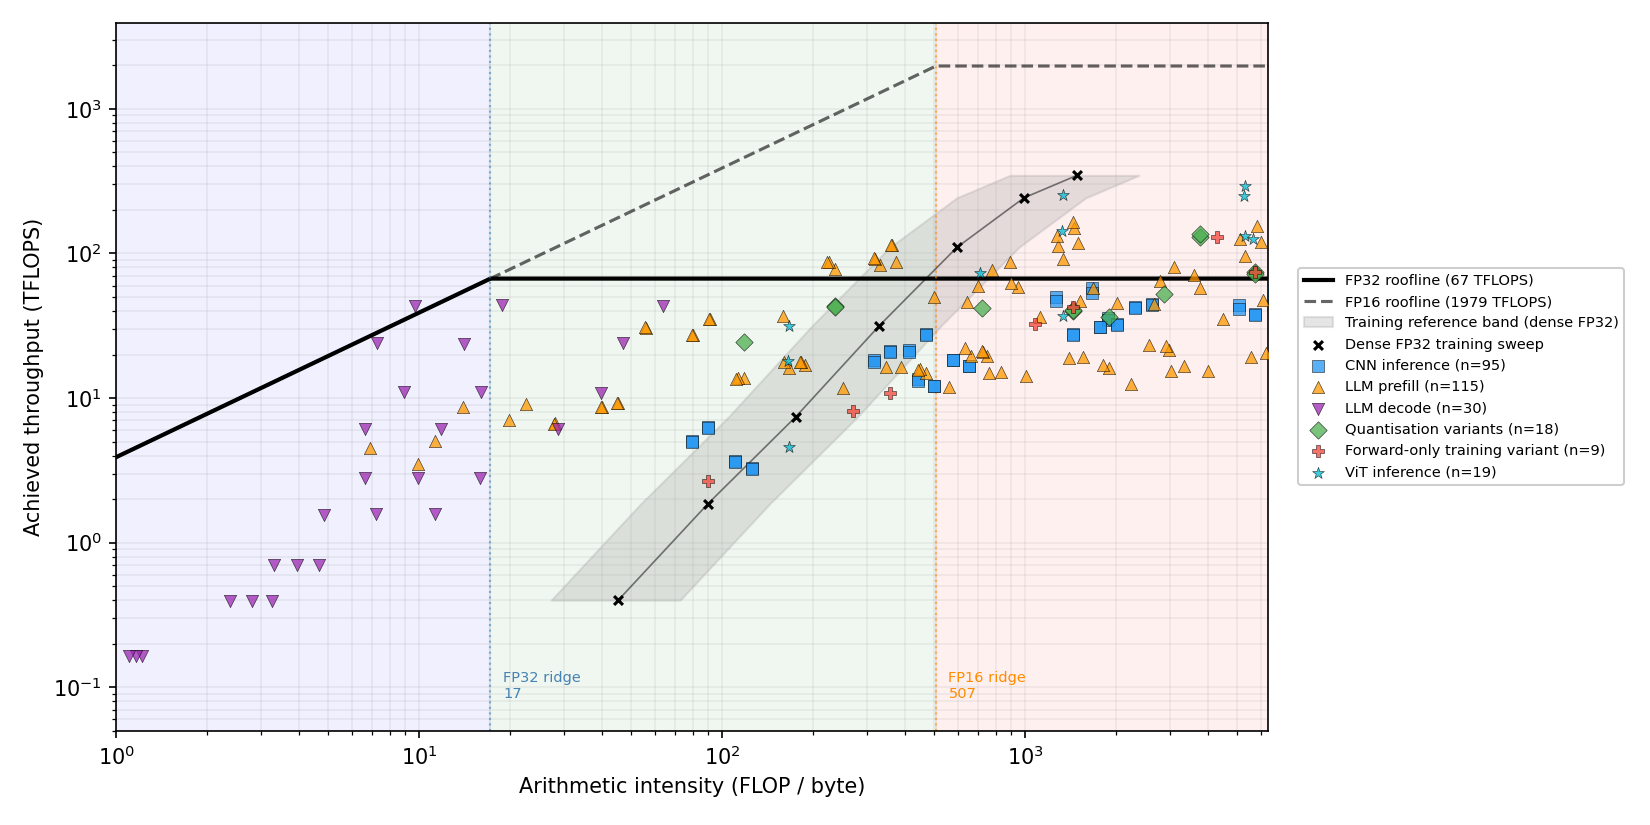
\includegraphics[width=0.88\linewidth]{figs/roofline_corner_cases.png}
\caption{H100-NVL roofline with the 286 corner-case inference configurations overlaid on a dense-FP32 training reference sweep. Color-coded by workload family (CNN inference, LLM prefill, LLM decode, quantisation variants, forward-only training variant, ViT inference). The CNN-inference, LLM-prefill, and quantisation clouds land squarely inside the training AI band, confirming visually that static heuristics cannot separate these inference workloads from training.}
\label{fig:roofline}
\end{figure}

\section{Window Size vs Accuracy}
\label{sec:window}

Classification accuracy is compared across 5/10/15/20/30/45/60/90/120 s windows. Detection is fairly flat (97.91--99.18\%), so shrinking the window size to 5 s would cost barely 1\% in performance. This means that a monitoring system can be configured to operate with very quick latency without significant accuracy loss.

\begin{figure}[htbp]
\centering
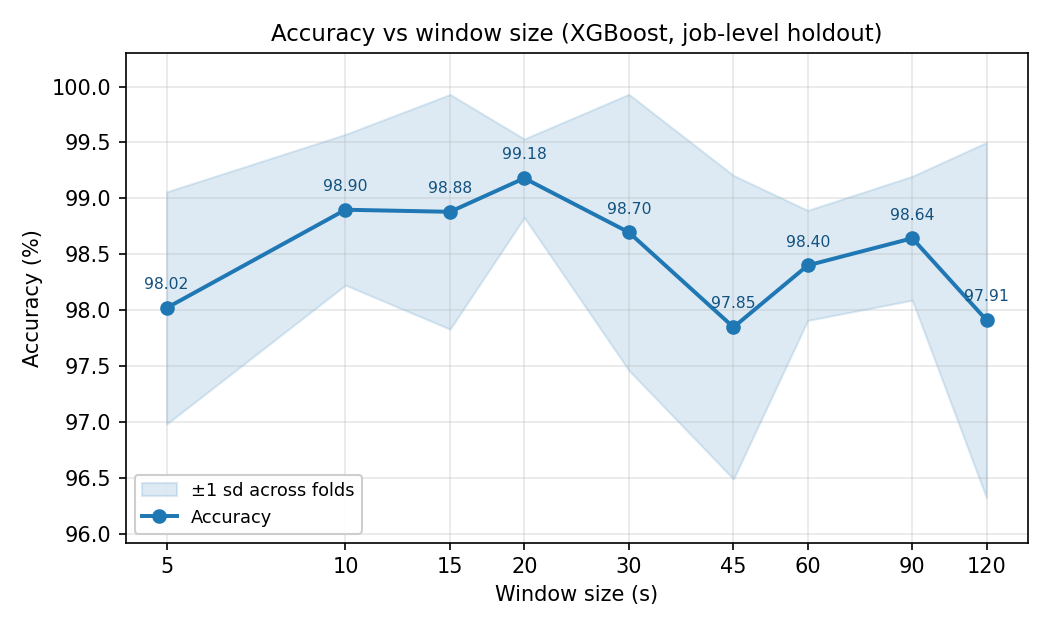
\includegraphics[width=0.80\linewidth]{figs/accuracy_vs_window_xgb.png}
\caption{accuracy vs window size.}
\label{fig:window}
\end{figure}

\section{Holdout Methodologies}
\label{sec:holdout}

We compare three different protocols for splitting the windows in the dataset into training and test sets and evaluating the classifier. The three protocols differ in how they group traces within the dataset, and in what questions they answer. Our corpus contains 1,558 runs from 1,198 jobs in 194 families.

\begin{itemize}\itemsep2pt
  \item \textbf{Run-level} holdout groups all windows from a run together, where a run is the telemetry transcript of a GPU from the beginning to the end of its job. Jobs can run on multiple GPUs, so under run-level holdout, it is possible for data from one GPU to appear in train and another GPU to appear in test. Since traces from different GPUs running the same job are often nearly identical, this would contaminate the test set, so we do not use it.
  \item \textbf{Job-level} holdout groups all traces from a job together, where a job is the combined execution of a workload program on some number of GPUs (in this study, 1--8). Our corpus sometimes contains multiple jobs that are variations on the same workload, so a classifier evaluated under job-level holdout on a particular job may have seen a different variation of that job in training, but never the specific job it is being tested on. This is the main protocol reported in this study.
  \item \textbf{Family-level} holdout groups all jobs from a family of workloads together; for example, if one adversarial job diluted training 50:50 with inference and another job did the same training and inference but in a 20:80 ratio, both jobs are within the same family. This is the most important measurement for understanding generalization to completely novel workloads, and we report it whenever making claims about generalization.
\end{itemize}

\subsection{Comparison of results by protocol}

The headline result is demonstrated here, calculated using a random forest under each protocol. Each figure is the mean over five fold-assignment seeds with the forest seed held fixed; the interval is one standard deviation across those seeds.

\begin{table}[htbp]
\centering
\footnotesize
\begin{tabular}{lrrrrrr}
\toprule
\textbf{protocol} & \textbf{groups} & \textbf{jobs split} & \textbf{accuracy} & \textbf{precision} & \textbf{recall} & \textbf{specificity} \\
\midrule
run-level & 1,477 & 245 & 99.15 $\pm$ 0.15 & 99.33 $\pm$ 0.18 & 99.20 $\pm$ 0.13 & 99.10 $\pm$ 0.25 \\
job-level & 1,116 & 0 & 97.66 $\pm$ 0.37 & 97.21 $\pm$ 0.24 & 98.37 $\pm$ 0.98 & 96.22 $\pm$ 0.35 \\
family-level & 161 & 0 & 86.34 $\pm$ 1.91 & 82.83 $\pm$ 1.05 & 97.19 $\pm$ 0.55 & 72.95 $\pm$ 1.95 \\
\bottomrule
\end{tabular}
\caption{random forest classifier performance metrics evaluated under each telemetry grouping protocol for cross-validation.}
\label{tab:protocol}
\end{table}

The important structure in this table is not the accuracy column. Recall is nearly invariant across the three protocols, spanning 97.19\% to 99.20\%, while specificity falls from 99.10\% to 72.95\%. The choice of protocol does not widely change whether the detector recognises training it has not seen; it changes how often the detector mistakes unfamiliar honest work for training. The eleven-point accuracy gap between run-level and family-level grouping is almost entirely driven by false positives under family-level holdout.

These false positives are concentrated rather than diffuse. Under family-level holdout, the fifteen worst benign cells account for 98.9\% of all false positives, and two cells account for 54\% of them. False-positive rates under job-level and family-level grouping, for the eight largest contributors:

\begin{table}[htbp]
\centering
\footnotesize
\begin{tabular}{llrrr}
\toprule
\textbf{Cell} & \textbf{Class} & \textbf{Windows} & \textbf{FP Job-level} & \textbf{FP Family-level} \\
\midrule
mining\_ethash\_proxy & non-ML & 1,255 & 0.0\% & 81.5\% \\
resnet50\_inference & inference & 1,022 & 0.0\% & 100.0\% \\
llm\_infer\_deepseek\_v3\_tp8 & inference & 1,272 & 25.2\% & 39.2\% \\
llm\_infer\_sdxl & inference & 327 & 4.6\% & 91.4\% \\
llm\_infer\_mistral\_7b\_q4 & inference & 503 & 3.0\% & 43.9\% \\
rendering\_proxy & non-ML & 1,021 & 0.0\% & 17.4\% \\
blender\_bmw & non-ML & 169 & 1.2\% & 76.9\% \\
whisper\_inference & inference & 117 & 0.9\% & 97.4\% \\
\bottomrule
\end{tabular}
\caption{false-positive rates across eight benign families highlighted for their difficulty to distinguish from training.}
\label{tab:fp}
\end{table}

Aggregated by class, inference workloads go from 4.3\% to 27.0\% false positives and non-ML GPU work from 1.1\% to 28.5\%. The two failure modes are sustained non-ML compute (mining and rendering proxies, Blender) and large-model inference, which are precisely the workloads a shared research cluster contains in quantity. A deployment facing a workload mix the detector was not fitted on should expect roughly one false alarm in four on those classes.

\subsection{Which protocol to use}

Job-level grouping is the main-body protocol. It is the strictest partition with no measured leakage, and it matches the unit an operator actually monitors: a job, not an individual GPU stream.

Family-level grouping answers the harder question of whether the detector generalises to a workload family it has never encountered. We report it wherever a generalisation claim is made, and it is the figure a reader should use when estimating false-alarm load on an unfamiliar cluster.

Run-level grouping splits 245 jobs across its folds, so it is not used and should not be read as an estimate of deployed performance.

\section{Job-Level Evaluation}
\label{sec:joblevel}

Results reported elsewhere in the paper concern classification of \emph{windows} from jobs of unknown workload type, but ultimately, the governing authority needs to know the category of the whole job. Therefore, we evaluate further statistics and methods on job-level classification.

\subsection{Setup and operating point}

Every figure in this section comes from the same corpus and classifier as the main results: 36,666 windows from 1,558 runs across 1,198 jobs, 30 s windows at 15 s stride, XGBoost, scored out of fold under 5-fold cross-validation grouped by job, so no run is ever scored by a model that saw its own job. Results are averaged over five fold-assignment seeds and reported as mean $\pm$ standard deviation.

\textbf{Window-level reference.} The per-window detector reaches ROC AUC 0.9993 $\pm$ 0.0005 and average precision 0.9995 $\pm$ 0.0003, with expected calibration error 0.0046 over ten equal-width bins. At the operating threshold $\tau$ = 0.75 it flags 98.14\% $\pm$ 0.63\% of training windows and 0.58\% $\pm$ 0.25\% of non-training windows.

\textbf{Aggregation rule.} We flag a run as training when 3 of any 5 consecutive windows exceed $\tau$ = 0.75. The rule is causal, using only windows that have already closed, so its alert time is a quantity an operator would actually observe. The false-alert pool is every non-training run in the corpus: 606 runs totalling 65.6 run-hours.

\begin{table}[htbp]
\centering
\footnotesize
\begin{tabular}{@{}L{0.21}L{0.12}L{0.08}L{0.13}L{0.12}L{0.12}@{}}
\toprule
\textbf{Rule} & \textbf{Detection} & \textbf{Missed runs} & \textbf{False alerts per benign run} & \textbf{False alerts per run-hour} & \textbf{Median time to first alert} \\
\midrule
3-of-5 at $\tau$ = 0.75 & 85.61\% $\pm$ 0.44 & 14.39\% & 1.19\% & 0.110 & 60 s \\
CUSUM at matched false alarms & 81.43\% $\pm$ 1.31 & 18.57\% & 1.12\% & 0.104 & 84 s \\
Either rule (hybrid) & 85.82\% $\pm$ 0.27 & 14.18\% & 1.35\% & 0.125 & 60 s \\
\bottomrule
\end{tabular}
\caption{Run-level alert rules at a fixed operating point. A run is flagged when 3 of any 5 consecutive 30 s windows exceed $\tau$ = 0.75; CUSUM accumulates P(training) - 0.25 per window and fires at h = 2.75, chosen so its benign false-alert rate does not exceed the 3-of-5 rule's on the same runs. Detection and false alerts are means over five fold-assignment seeds; the false-alert pool is 606 non-training runs totalling 65.6 run-hours.}
\label{tab:rules}
\end{table}

Short runs account for almost all of the misses. Of the 134 training runs the 3-of-5 rule fails to flag, 130 contain fewer than three windows, which is fewer than the rule needs to fire at all: a run shorter than about 60 s of telemetry cannot produce three closed windows. Conditional on a run being long enough for the rule to be able to fire, detection is 99.5\% (818 of 822). By run length, detection is 0\% at 1--2 windows, 96.1\% at 3--4, 100\% at 5--9, 99.1\% at 10--19, and 100\% at 20--49 and beyond. The missed runs are ordinary short fine-tuning jobs --- bert\_sst2, gpt2\_wikitext2 and resnet\_cifar10 variants account for 85 of the 134 --- and only two of them belong to an evasion family. The headline 14.4\% is therefore a statement about how short some of our runs are rather than about how well the detector works, and an operator monitoring jobs that last minutes rather than seconds should expect the conditional figure.

\textbf{Latency.} Median time to first alert is 60 s, the 95th percentile is 60 s, and the maximum is 474 s; 97.2\% of flagged runs alert within 60 s and 99.8\% within five minutes. The 60 s median is a structural floor rather than a measurement, since a rule requiring three closed 30 s windows at 15 s stride cannot fire sooner. This reconciles the two latency figures quoted during review: the 7 s figure described a single window crossing the threshold, which is not the rule we deploy, and 60 s is correct for the 3-of-5 rule.

\subsection{Separability by evasion family}

Figure~\ref{fig:runlevel} plots ROC and precision-recall for each evasion family against the full non-training window pool. Separability is high everywhere: ROC AUC is at least 0.9965 for every family and exactly 1.0000 for fifteen of the twenty-two. The hard families are distinguished by average precision rather than by AUC --- whitebox\_lora 0.9000, symgemm\_L4\_fused\_sgd 0.9571, I\_stochastic 0.9666 and K\_online\_learning 0.9794, against at least 0.9958 for every other family. True positive rate at a 1\% false positive rate is 0.920 for symgemm\_L4\_fused\_sgd, 0.971 for I\_stochastic, 0.980 for K\_online\_learning, and 1.000 for the rest. The classifier therefore separates every family we constructed from benign activity, and the difficulty in the hard cases is threshold placement, not separability.

\subsection{A memoryful alert rule}

The 3-of-5 trigger is memoryless: evidence that never clears $\tau$ in any single window is discarded no matter how long it persists. That is exactly the wrong property for a disguise that holds P(training) consistently just below the threshold, which is what the symmetric-GEMM and white-box LoRA strategies do. We therefore also evaluate a one-sided cumulative sum: $S_0 = 0$, $S_t = \max(0,\, S_{t-1} + p_t - k)$ with reference k = 0.25, alerting when $S_t \geq h$. Inference runs drift the statistic to zero; training runs accumulate.

\textbf{Calibration.} We set h to the smallest value whose realised false-alert rate on benign runs is no worse than the 3-of-5 rule's own rate on the same runs, giving h = 2.75 (2.75--3.75 across seeds). Matching false alarms rather than choosing a round number is what makes the comparison meaningful: a sequential test with a free threshold can always be made to look better than a fixed one.

In distribution, CUSUM does not help. It detects 81.43\% of training runs against the 3-of-5 rule's 85.61\%, and its median latency is 84 s rather than 60 s. Both gaps have the same cause as the misses above --- accumulating to h = 2.75 takes about four windows, so CUSUM arms more slowly than a 3-of-5 rule and fires on only 31.4\% of runs that are 3--4 windows long, against 96.1\% for 3-of-5. On runs of five windows or more the two rules are both at 100\%.

\subsection{Transfer to unseen strategies}

The case the rules actually differ on is a family the detector has never trained on. We refit excluding one evasion family at a time and apply both rules at the thresholds calibrated above, changing nothing else. CUSUM never does worse on any of the twenty-two families, and improves four of them --- every one of which is a family the memoryless rule struggles with.

\begin{table}[htbp]
\centering
\footnotesize
\begin{tabular}{lrrrrr}
\toprule
\textbf{Family (held out)} & \textbf{Mean window P(training)} & \textbf{Windows above $\tau$} & \textbf{3-of-5} & \textbf{CUSUM} & \textbf{Hybrid} \\
\midrule
symgemm\_L4\_fused\_sgd & 0.107 & 2.7\% & 8.3\% & 25.0\% & 25.0\% \\
whitebox\_lora & 0.504 & 40.0\% & 50.0\% & 83.3\% & 83.3\% \\
O\_composite\_idle\_pad & 0.780 & 69.2\% & 71.9\% & 79.7\% & 81.2\% \\
whitebox\_full & 0.802 & 66.5\% & 87.5\% & 100.0\% & 100.0\% \\
B\_low\_util & 0.661 & 66.8\% & 70.0\% & 70.0\% & 70.0\% \\
K\_online\_learning & 0.944 & 93.1\% & 94.4\% & 94.4\% & 94.4\% \\
Mean over all 22 families & --- & --- & 90.1\% & 93.3\% & 93.4\% \\
\bottomrule
\end{tabular}
\caption{Transfer to unseen evasion families. The classifier is refit with one evasion family held out entirely, then both rules are applied at the thresholds calibrated in Table~\ref{tab:rules} with nothing else changed. Only the six families below 100\% are listed; the remaining sixteen are flagged on every run by both rules. CUSUM is never worse than the 3-of-5 rule on any family.}
\label{tab:transfer}
\end{table}

The remaining sixteen families are flagged on every run by both rules. The pattern is consistent with the motivation: where the per-window evidence is weak but persistent, accumulating it recovers detections that thresholding discards. The fused-write kernel, the hardest workload in the corpus, triples from 8.3\% to 25.0\%, and white-box LoRA rises from 50.0\% to 83.3\%. Latency is the cost --- median time to first alert under CUSUM on these families is 150 s for the fused-write kernel and 240 s for white-box LoRA, against the 60--90 s typical elsewhere --- which is the expected trade for a rule that waits for evidence to accumulate.

There are two caveats. First, 25.0\% run-level detection of an unseen fused-write kernel is better than 8.3\% but it is not a deployable detection rate; the honest reading is that a memoryful rule narrows the gap rather than closing it. Second, successive windows overlap and are highly autocorrelated --- we measure pairwise correlations above 0.97 at separations from 30 s to 4 h --- so a long run supplies far less independent evidence than its window count suggests, and a CUSUM threshold chosen on independence assumptions would be badly miscalibrated. Calibrating h on benign runs that carry the same correlation structure is what keeps the comparison honest, and it is why we report a matched-false-alarm comparison rather than a matched-h one.

\begin{figure}[htbp]
\centering
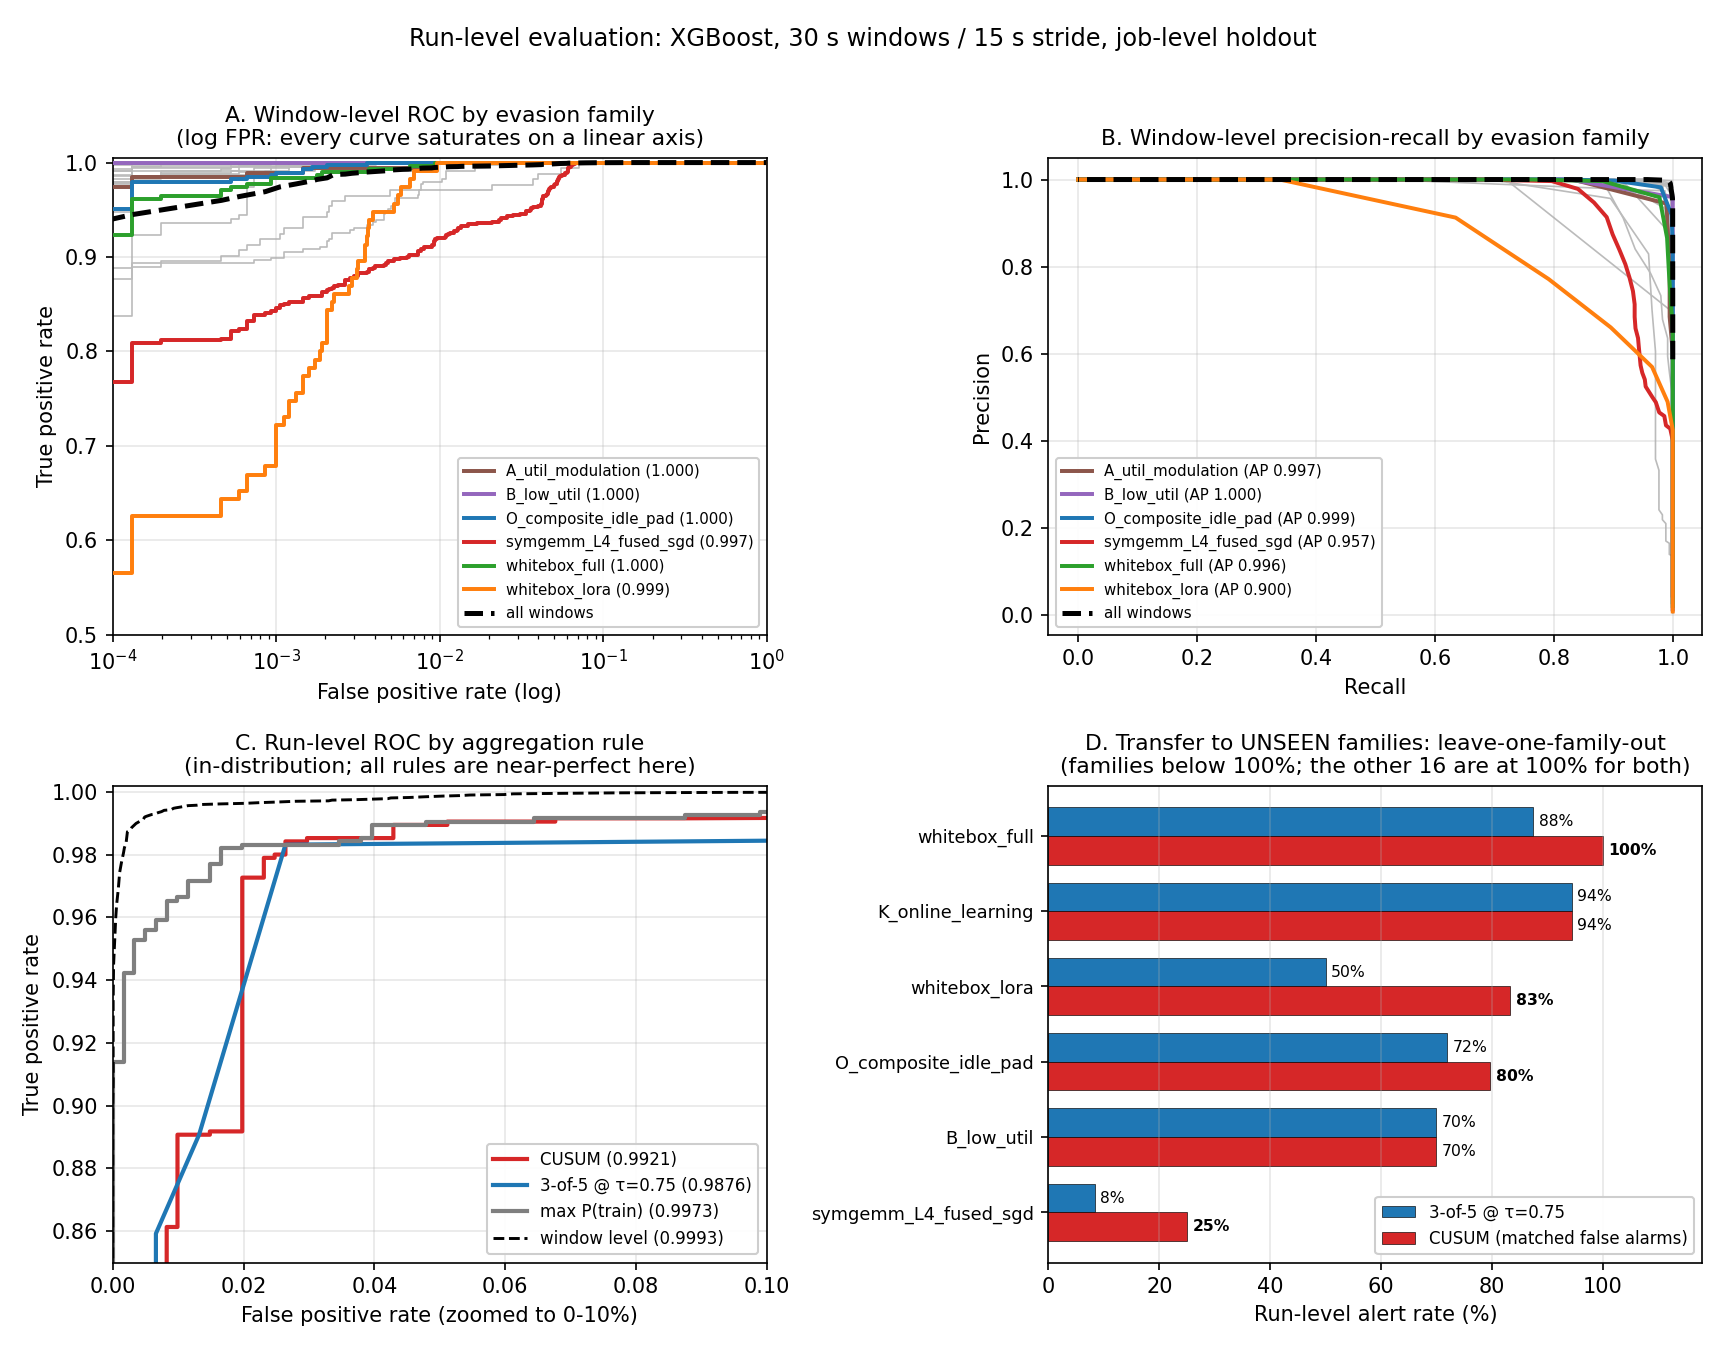
\includegraphics[width=0.95\linewidth]{figs/runlevel_roc_pr_xgb.png}
\caption{run-level evaluation (runlevel\_roc\_pr\_xgb.\{png,pdf\}). A: window-level ROC by evasion family, on a logarithmic false-positive axis because every curve saturates on a linear one. B: window-level precision-recall by family; whitebox\_lora and symgemm\_L4\_fused\_sgd are the two visibly below the rest. C: run-level ROC for each aggregation rule, zoomed to the first 10\% of false-positive rate. D: leave-one-family-out alert rates for the six families below 100\%, comparing the memoryless 3-of-5 rule with CUSUM at matched false alarms; the other sixteen families are at 100\% under both.}
\label{fig:runlevel}
\end{figure}

\section{Additional Results}

Here we compare the 22 adversarial evasion strategies, sorted by detection rate in leave-one-out evaluation.

\begin{figure}[htbp]
\centering
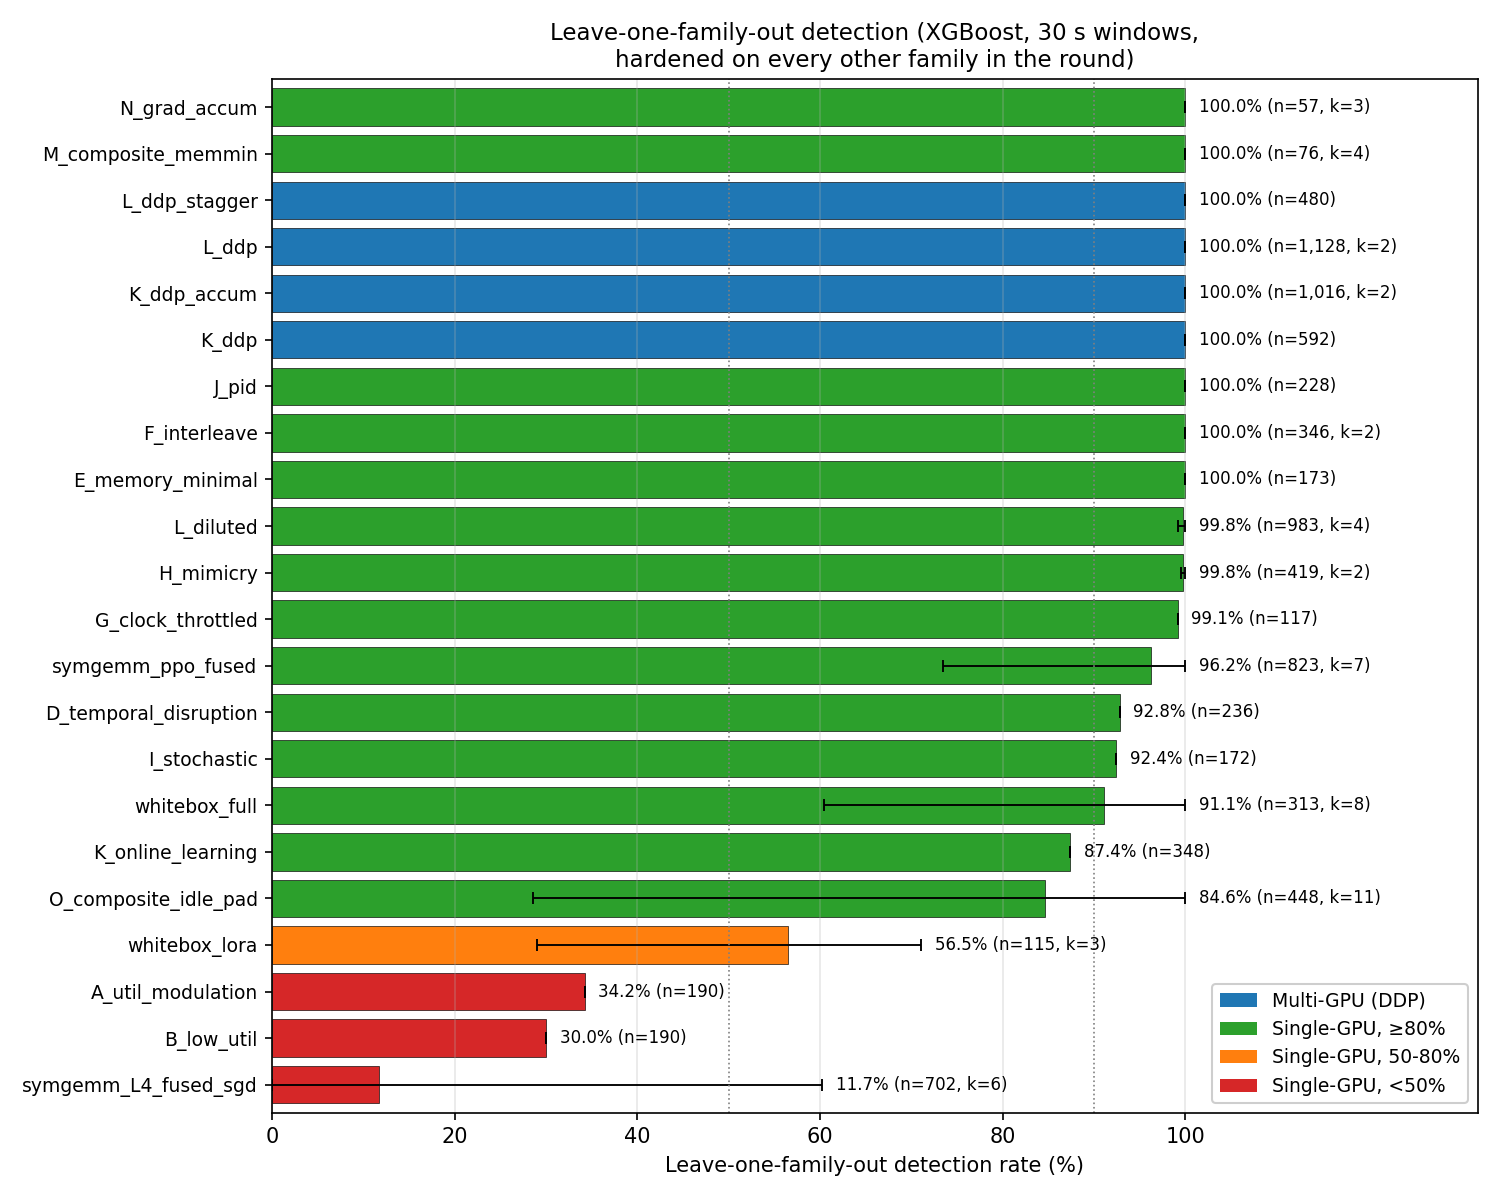
\includegraphics[width=0.92\linewidth]{figs/loo_detection_bar_xgb.png}
\caption{detection rate in LOO evaluation by strategy family. Error bars show min/max across variants within each family.}
\label{fig:loo}
\end{figure}

\section{Telemetry Visualizations}

Here is a visual representation of some telemetry features transcribed from selected workloads.

\begin{figure}[htbp]
\centering
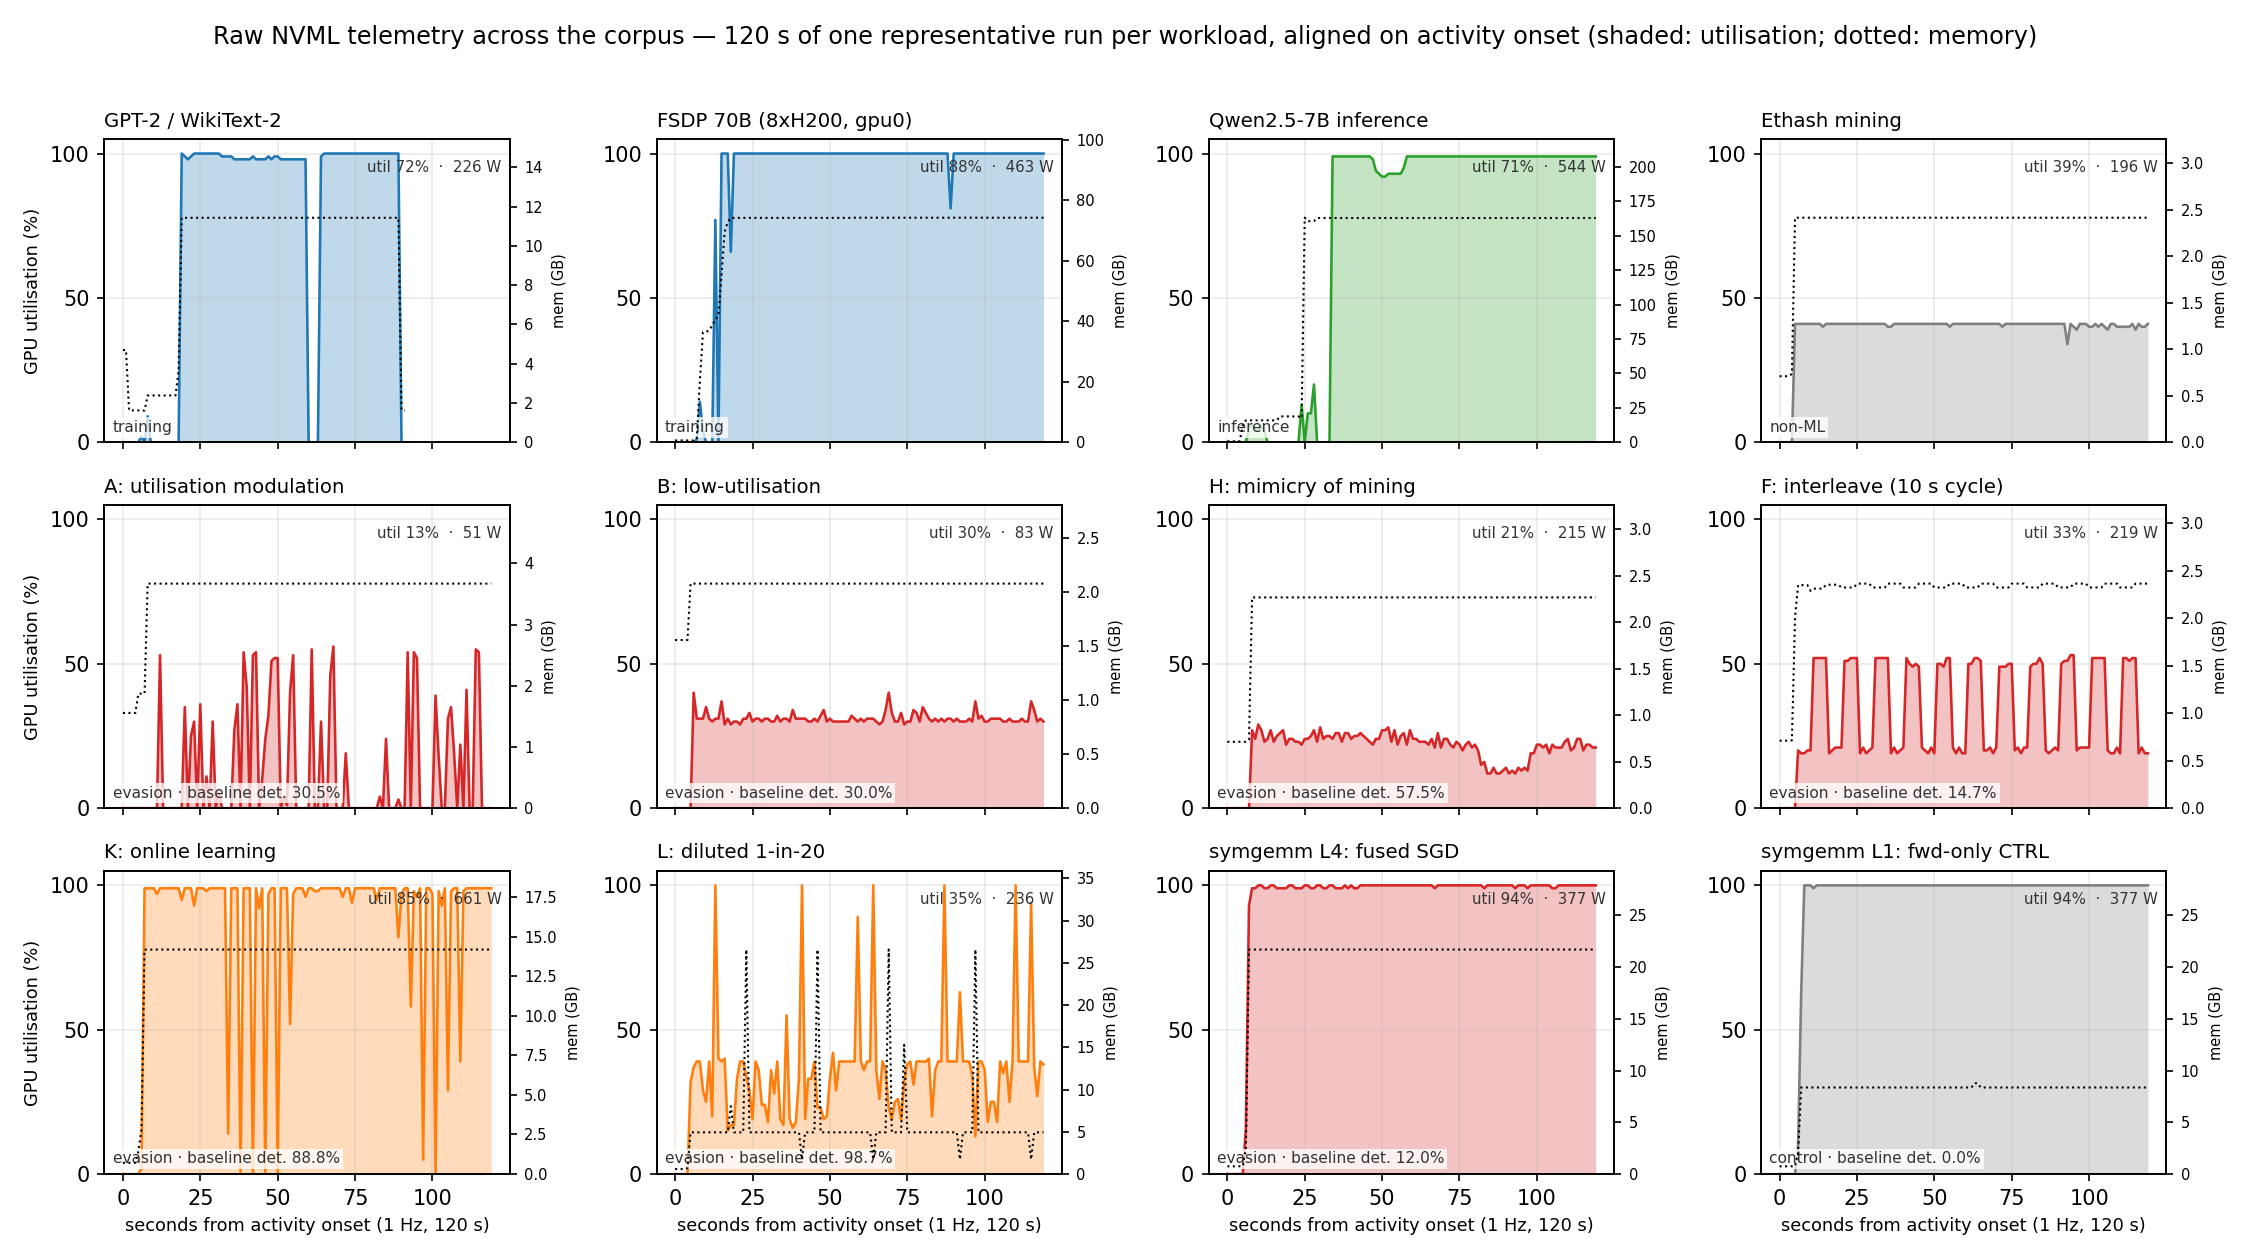
\includegraphics[width=0.98\linewidth]{figs/telemetry_catalog.png}
\caption{raw NVML telemetry for twelve workloads, 120 s per panel at 1 Hz, aligned on activity onset. Shaded area is GPU utilization (left axis), dotted line is memory in GB (right axis). Adversarial panels are labeled with their baseline detection rate from Table~\ref{tab:catalog}. The last two panels illustrate a matched pair: symgemm\_L4\_fused\_sgd is disguised training, symgemm\_L1\_fwd3 is a similar forward-only workload, and their only difference is memory.}
\label{fig:catalog}
\end{figure}

\section{Limitations and Future Work}
\label{sec:limits}

This work has several limitations. First, our experiments were conducted exclusively on single-node hardware configurations, testing workloads on instances up to only 8 GPUs. Future experiments should expand to greater GPU counts, including multi-node clusters. Evasion characteristics for multi-node model- and data-parallel training will differ due to different types of interconnect (such as InfiniBand between servers vs NVLink within servers), but it is likely that training will continue to be highly distinctive due to the communication requirements of large-scale training. Relatedly, model sizes were limited by memory constraints, with largest usable models of 70B parameters for training and 671B MoE for inference. Today's frontier models are often much larger and can require more than 8 GPUs to train and serve.

Second, our adversarial strategies were limited to framework-level evasion implemented in pytorch. An adversary with access to custom CUDA kernels could potentially manipulate individual kernel behavior, which we did not test. Future research should investigate the effectiveness of these strategies and see how robust the classifier becomes against them.

Third, the integrity of the telemetry channel is a critical assumption. Our evaluation assumes the adversary cannot tamper with NVML readings or performance counter values, nor inject synthetic telemetry to spoof a workload signature. These guarantees require a HEM for tamper-resistant telemetry and an authenticated channel. Other work like \citet{monfared2026} investigates what can be done if these guarantees are not available.

Fourth, we only tested on NVIDIA GPUs released since 2020. This category includes the large majority of compute capacity available to cloud tenants, but substantial amounts of other chips exist, including AMD and Huawei GPUs and custom silicon such as Google TPUs and Amazon Inferentia and Trainium \citep{epoch2025}. Future work should generalize this approach using the analogous telemetry signals available for other hardware.

Fifth, our telemetry was sampled at \textasciitilde{}1 Hz, a frequency which cannot detect very brief events. Future work should test other sampling rates, measuring how much classification improves with more frequent sampling, how much sampling can be done without degrading performance, and investigating the minimum sample rate that is still difficult to evade.

Finally, we only tested a limited range of workloads and adversarial strategies. Real datacenters run a wider variety of applications than we emulated, with notable gaps including multi-user inference serving, data processing and ETL pipelines, and predictive analytics. Although we tried to cover many evasion strategies and edge cases, real evaders might attempt a much wider range of tactics that we cannot anticipate. It is important to continue iterating on this work to make the classifier even more robust to unknown future threats. Iteration should include more white-box rounds, to determine whether resistance to white-box attacks improves generally, or if an evader can always defeat a classifier if they obtain white-box access, and if so, how much performance penalty is incurred in the process.
